\documentclass{article}

\usepackage[latin1]{inputenc}
\usepackage[T1]{fontenc}
\usepackage{amsmath}
\usepackage{multicol}
\usepackage{graphics}


\begin{document}
	\begin{figure}[!h]
		% 30% de la página
		\begin{minipage}[b]{0.3\textwidth}
			La imagen de la derecha muestra un icosaedro junto con un
			dodecaedro (figura central), los satélites son un icosaedro,
			un dodecaedro y un tetraedro. Las figuras fueron generadas con
			{\sc Mathematica} y maquilladas con {\it Inkscape}.
			% 60% de la pág
		\end{minipage} \hfill \begin{minipage}[b]{0.6\textwidth}
		\begin{center}% Figuras: ver capítulo 5
			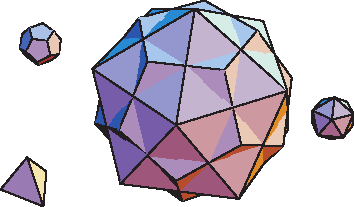
\includegraphics{images/ML_fig3.pdf}
			\caption{ Poliedros}
		\end{center}
	\end{minipage}
\end{figure}
\end{document}
